\documentclass[10pt,a4paper]{article}
\usepackage[utf8]{inputenc}
\usepackage[polish]{babel}
\usepackage[T1]{fontenc}
\usepackage{amsmath}
\usepackage{amsfonts}
\usepackage{amssymb}
\usepackage{graphicx}
\usepackage{epsf} 
\usepackage{float}
\nonstopmode

\title{Flow-Shop Scheduling\\Laboratorium Optymalizacji Kombinatorycznej}

\author{Szymon Gramza\\
  szymon.gramza@student.put.poznan.pl
\and
  Maciej Sobkowski\\
  maciej.sobkowski@student.put.poznan.pl
\and
  Prowadzący: Marcin Radom
}

\begin{document}
\maketitle
\section{Wprowadzenie}
\subsection{Opis problemu}
Problem Flow-Shop jest problemem optymalizacji kobminatorycznej, który polega na
szeregowaniu zadań przy wykorzystaniu ustalonej liczby maszyn. Każde zadanie
składa się z listy operacji, które muszą zostać wykonane w określonej kolejności
na określonej maszynie, a każdą operację cechuje czas wykonywania. Zadania
pojawiają się w różnych momentach pracy systemu, a maszyny na których są
wykonywane posiadają wymuszone przestoje.  Do rozwiązania powyższego problemu
wykorzystaliśmy zainspirowaną zachowaniem się mrówek poszukujących pożywienia
metaheurystykę ACO\@. Algorytm mrówkowy będziemy porównywać z rozwiązaniem
uzyskanym za pomocą algorytmów losowego oraz rozwiązaniem optymalnym obliczonym
za pomocą wzoru: 
\[ opt = \frac{\text{suma\ czasów\ wszystkich
operacji}}{\text{liczba\ maszyn}} \]

\subsection{Program testujący}

\subsubsection{Opis}
Aplikacja została napisana w języku C i wykorzystuje biblioteki dostępne w
systemach z rodziny GNU/Linux. 

\subsubsection{Kompilacja}
Kompilacja została zautomatyzowana przy pomocy programu GNU Make. Aby
skompilować program należy przejść do katalogu \textit{scheduler} i z poziomu 
konsoli wydać polecenie \textit{make}. Prawidłowe zakończenie procesu kompilacji 
zostanie zasygnalizowane komunikatem \textit{Zakończono linkowanie!}. W ten sam
sposób należy przebiega kompilacja programu \textit{generator}.

\subsubsection{Uruchomienie}
Praca aplikacji jest sterowana przez przełączniki powszechnie stosowane w
oprogramowaniu linuksowym.  Przykładowe wywołanie \textit{scheduler -i
inst\_name -o file\_name.csv} uruchomi program dla instancji zapisanej w pliku
inst\_name i wykona algorytm ACO oraz losowy. Wynik szeregowania zostanie
zapisany do pliku o nazwie file\_name.csv.  Dodatkowo, aby uruchomić program
generujący instancje należy użyć polecenia \textit{./generator}.\\ Przykładowe wywołanie:
\textit{./generator -i input\_name -o inst\_name } spowoduje wygenerowanie pliku
instancji inst\_name przyjmując parametry zawarte w pliku input\_name zgodnie ze
schematem, że każda linia składa się z 5 liczb całkowitych, które odpowiednio
charakteryzują: liczbę zadań, początek i koniec przedziału czasu wykonania
operacji, początek i koniec przedziału czasu gotowości zadania.\\ Generator
losuje czasy wykonania operacji i czasy gotowości dla zdefiniowanej liczby
zadań.

\section{Algorytm Ant Colony Optimization}

\subsection{Opis algorytmu}
Zastosowana przez nas metaheurystyka - Ant Colony Optimization - opiera się na
naturalnym zachowaniu kolonii mrówek poszukujących pożywienia. Algorytm korzysta
ze struktur utrzymujących informację o drodze od źródła do celu, przebytej przez
każdą mrówkę danego pokolenia. Algorytm został zaprojektowany do problemów
znajdowania ścieżki w grafie o najmniejszym koszcie (problem TSP).
Przystosowanie algorytmu do problemu szeregowania zadań sprowadza się w naszym
przypadku do przedstawienia operacji danej instancji w postaci grafu, którego
przykład umieszczono poniżej:\\
\begin{center}
    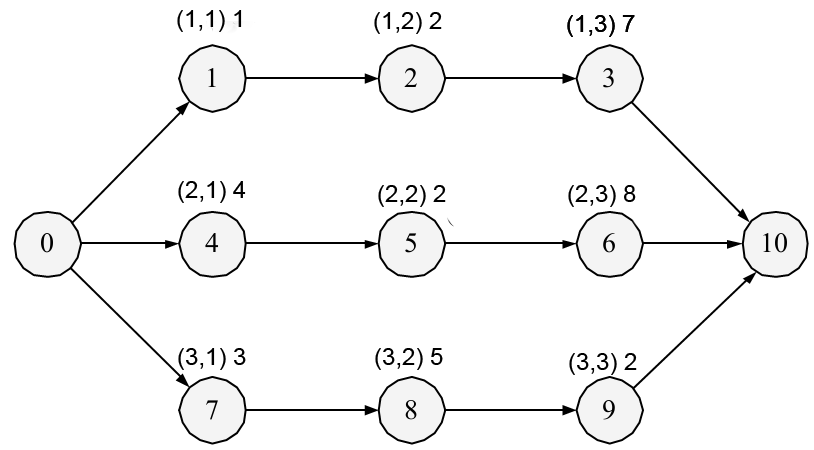
\includegraphics[scale=0.4]{./figures/pic01.png}\\
\end{center}
Każdemu wierzchołkowi grafu przyporządkowana jest jedna operacja, każda
operacja zaś posiada informacje o maszynie i numerze zadania.  Zależności
pomiędzy kolejnością wykonania operacji reprezentują łuki między nimi, ponadto
graf posiado dwa dodatkowe wierzchołki - początkowy i końcowy - które pozwalają
przypisać pierwszej i ostatniej operacji feromon. Dzięki takiej reprezentacji
problemu możemy korzystać z wzorów przeznaczonych dla algorytmu TSP z drobnymi
modyfikacjami.

Informacje o ilości feromonów utrzymywane są w macierzy NxN (N - liczba
operacji).  Rozwiązaniem generowanym przez mrówkę jest łańcuch wszystkich
wierzchołków zachowujący zależnosci między operacjami w zadaniu.  (sortowanie
topologiczne) Przykładowy łańcuch: [0 1 4 2 7 5 8 3 6 9 10].

Przed uruchomieniam właściwego algorytmu, początkowa ilość feromonu na każdej
ścieżce przyjmuje bardzo małą wartość, w naszej implementacji przyjęliśmy $
\tau_0 = 0.001 $ 

\subsubsection{State Transition Rule}
Każda mrówka wybierając drogę stosuję regułę zmiany stanu (State Transition
Rule), którą obrazuje poniższy wzór:\\

\begin{equation}
 s = \left\{ 
  \begin{array}{l l}
    arg\ max_{u \in J(r)} \{ [\tau (r,u)] \cdot [\eta (r,u)^\beta] \} , & \quad
    \text{jeśli $q\leq q_0$}\\
    S, & \quad \text{w przeciwnym razie}
  \end{array} \right.
\end{equation} \\
gdzie:
\begin{itemize}
  \item $ (r,u) $ - łuk od wierzchołka r do u
  \item $ J(r) $ - zbiór wierzchołków dostępnych w punkcie decyzyjnym r
  \item $ \tau (r,u) $ - ilość feromonu na łuku (r,u)
  \item $ \eta (r,u) $ - atrakcyjność łuku (r,u), która w przypadku naszego
    problemu zdefiniowana jest jako odwrotność długości operacji u
  \item $ \beta $ - parametr kontrolujący wpływ atrakcyjności
  \item $ q $ - losowa liczba z przedziału $ \langle 0;1 \rangle $ 
  \item $ q_0 $ - zdefiniowany parametr przyjmujący wartości z przedziału $
    \langle 0;1 \rangle $
  \item $ S $ - zmienna losowa wybierana zgodnia z rozkładem prawdopodobieństwa
    opisanym wzorem (2). 
\end{itemize}
\\
\begin{equation}
 P(r,s) = \left\{ 
  \begin{array}{l l}
    \frac{[\tau (r,s)] \cdot [\eta (r,s)^\beta]}{\sum_{u \in J(r)} {[\tau (r,u)]
    \cdot [\eta (r,u)^\beta]}},
    & \quad \text{jeśli }s \in J(r)\\
     0, & \quad \text{w przeciwnym razie}
  \end{array} \right.
\end{equation}

Powyższa metoda wyboru nosi nazwę pseudoruletki, której zasada działania opiera
się na przydzieleniu wartości procentowej koła ruletki, odpowiadającej
iloczynowi ilości feromonu i atrakcyjności. Po zakręceniu kołem, które jest
równoważne wylosowaniu liczby, wybierany jest następny wierzchołek na drodze
mrówki.

\subsubsection{Aktualizacja wartości feromonów}
W algorytmie stosujemy dwie strategie aktualizacji feromonów: \\
\begin{enumerate}
  \item lokalna (local updating rule) - w czasie konstruowania ścieżki mrówka
    modyfikuje ilosć feromonu stosując się do poniższego wzoru:\\
  \[ \tau (r,s) \leftarrow (1 - \rho) \cdot \tau (r,s) + \rho \cdot \tau_0  \] \\
  gdzie:
  \begin{itemize}
  \item $ \rho $ - współczynnik parowania feromonu (z przedziału $ (0;1) $)
\end{itemize}

  \item globalna (global updating rule) - gdy wszystkie mrówki danej populacji
    dotrą do celu (osiągną końcowy wierzchołek grafu) wartość feromonu jest
    aktualizowana zgodnie ze wzorem:\\
   \[ \tau (r,s) \leftarrow (1 - \alpha) \cdot \tau (r,s) + \alpha \cdot \Delta \tau (r,s)  \] \\
  gdzie:
  \begin{itemize}
  \item $ \alpha $ - parametr zaniku feromonu
  \item $ \Delta \tau (r,s) $ - przedstawia się wzorem: \\
  \begin{equation}
 \Delta \tau (r,s) = \left\{ 
  \begin{array}{l l}
    (L_{gb})^{-1} , & \quad \text{jeśli $(r,s) \in$ najlepsza ścieżka}\\
    0, & \quad \text{w przeciwnym razie}
  \end{array} \right.
\end{equation}
  gdzie:
  \item $ L_{gb}$ - długość najlepszej ścieżki ($C_{max}$)
\end{itemize}
\end{enumerate}

\subsection{Instancje testowe}
Każda znajdująca się poniżej instancja sterowana jest następującymi
parametrami: $ \rho, \alpha, q_0, \tau_0, \beta $.  Klasy instancji
podzieliliśmy na 4 grupy w zależności od rodzaju danych wejściowych: losowe,
rosnące, malejące, v-kształtne.

\newpage
\subsubsection{Grupa instancji 1}
Różne klasy instancji danych wejściowych.

\begin{center}
\begin{tabular}{|r|l|}
  \hline
  liczba zadań & 50 \\
  czasy operacji & $ \langle 5;100 \rangle $  \\
  liczba mrówek & 10 \\
  liczba pokoleń & 5000 \\
  $ \rho $ & 0.01 \\
  $ \alpha $ & 0.1 \\
  $ q_0 $ & 0.8 \\
  $ \tau_0 $ & 0.001 \\
  $ \beta $ & 2 \\
  \hline
\end{tabular}
\end{center}

\begin{center}
\\
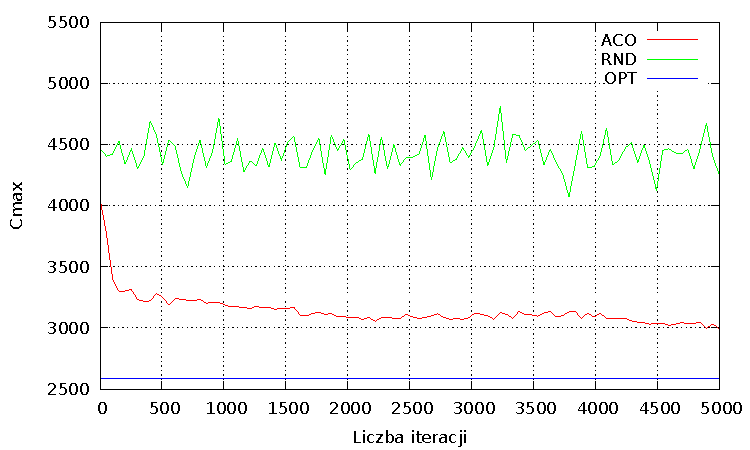
\includegraphics{./figures/inst01_rnd_smooth.pdf}
\caption{losowy}

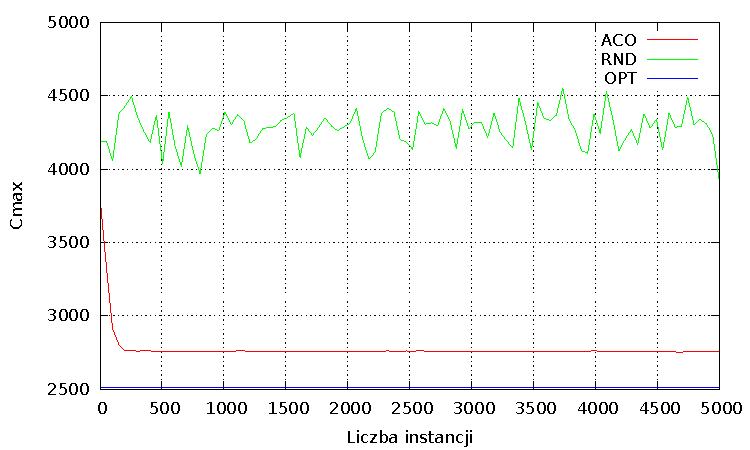
\includegraphics{./figures/inst02_asc_smooth.pdf}
\caption{rosnący}
\\
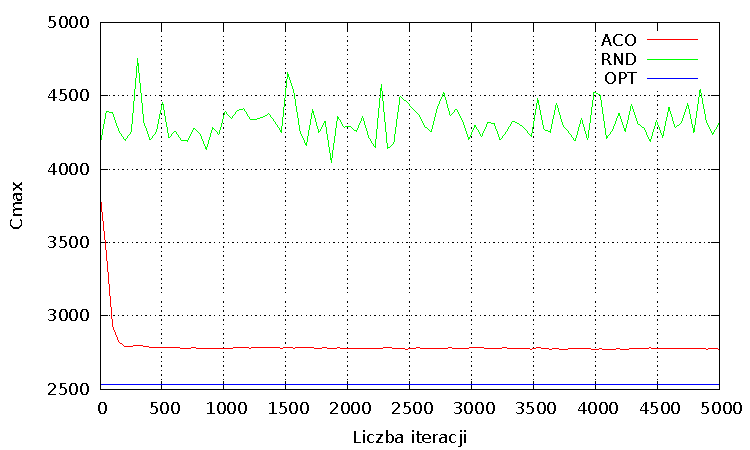
\includegraphics{./figures/inst03_dsc_smooth.pdf}
\caption{malejące}
\\
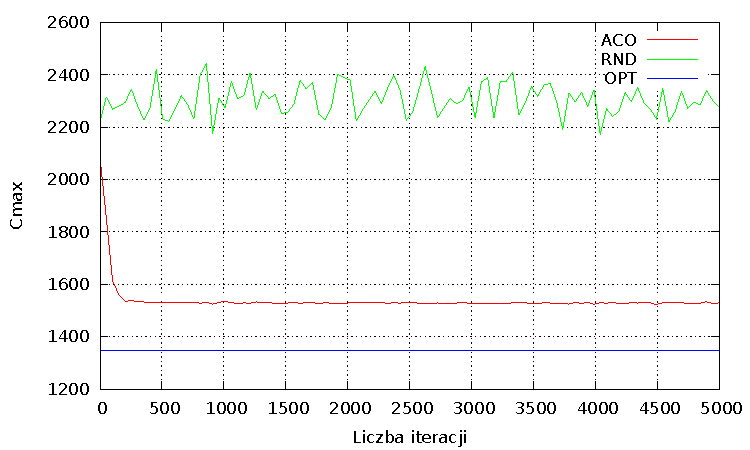
\includegraphics{./figures/inst04_vsh_smooth.pdf}
\caption{v-kształtne}
\\
\end{center}

Algorytm losowy, niezależnie od rodzaju danych wejściowych oraz ilości iteracji, osiąga średnio podobne wyniki. Jest to spowodowane brakiem poprawy algorytmu z upływem czasu. Natomiast ACO w kolejnych iteracjach zwraca wynik dążący do optimum.
Metaheurystyka w zależności od klasy instancji zwraca wynik procentowo?

\begin{tabular}{rrrll}
%\toprule
Iteracja & ACO & RND  & opt/ACO(\%) & opt/RND(\%) \\
%\midrule

50	& 3,796.33	& 4,294.33	& 68.03	& 60.14 \\
1000	& 3,192.15	& 4,419.17	& 80.91	& 58.44 \\
2000	& 3,089.85	& 4,388.67	& 83.59	& 58.85 \\
3000	& 3,101.63	& 4,331.83	& 83.27	& 59.62 \\
4000	& 3,077.53	& 4,458.83	& 83.92	& 57.92 \\
5000	& 3,016.63	& 4,238.50	& 85.61	& 60.93 \\
%\bottomrule
\end{tabular}

\begin{tabular}{rrrll}
%opt 2510.333
%\toprule
Iteracja & ACO & ASC  & opt/ACO(\%) & opt/ASC(\%) \\
%\midrule

50	& 3,397.37	& 4,300.33	& 73.89 &	58.38\\
1000	& 2,756.32	& 4,252.50 &	91.08 &	59.03\\
2000	& 2,757.57	& 4,480.17	& 91.03 & 56.03\\
3000	& 2,757.55	& 4,448.83	& 91.03 &	56.43\\
4000	& 2,757.02	& 4,457.83	& 91.05 &	56.31\\
5000	& 2,755.25	& 4,126.83	& 91.11 &	60.83\\
%\bottomrule
\end{tabular}

\begin{tabular}{rrrll}
%opt 2528.667
%\toprule
Iteracja & ACO & DSC  & opt/ACO(\%) & opt/DSC(\%) \\
%\midrule
50	& 3,418.53	& 4,367.67	& 73.97 &	57.90\\
1000	& 2,778.82	& 4,341.67	& 91.00 &	58.24\\
2000	& 2,780.03	& 4,394.00	& 90.96 & 57.55\\
3000	& 2,777.32	& 4,295.50	& 91.05 &	58.87\\
4000	& 2,770.00	& 4,411.33	& 91.29 &	57.32\\
5000	& 2,774.88	& 4,333.50	& 91.13 &	58.35\\

%\bottomrule
\end{tabular}

\begin{tabular}{rrrll}
%opt 1348.333
%\toprule
Iteracja & ACO & VSH  & opt/ACO(\%) & opt/VSH(\%) \\
%\midrule
50	& 1,859.73	& 2,282.00	& 72.50 &	59.09\\
1000	& 1,530.27	& 2,277.67	& 88.11 &	59.20\\
2000	& 1,529.47	& 2,341.00 &	88.16 &	57.60\\
3000	& 1,528.95	& 2,304.33 &	88.19 &	58.51\\
4000	& 1,529.55	& 2,340.17 &	88.15 &	57.62\\
5000	& 1,527.00	& 2,268.83 & 88.30 &	59.43\\

%\bottomrule
\end{tabular}

\newpage
\subsubsection{Grupa instancji 2}
Różne wartości parametru $\beta$.

\begin{center}
\begin{tabular}{|r|l|}
  \hline
  klasa instancji & losowa \\
  liczba zadań & 50 \\
  czasy operacji & $ \langle 5;100 \rangle $  \\
  liczba mrówek & 10 \\
  liczba pokoleń & 5000 \\
  $ \rho $ & 0.01 \\
  $ \alpha $ & 0.1 \\
  $ q_0 $ & 0.8 \\
  $ \tau_0 $ & 0.001 \\
  \hline
\end{tabular}
\end{center}

\begin{figure}[h]
    \centering
    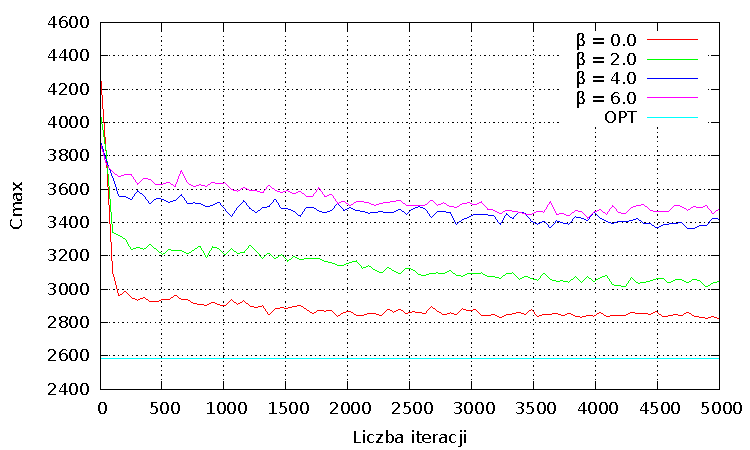
\includegraphics{./figures/inst01_rnd_beta_smooth.pdf}
    \caption{$ \beta = \{ 0, 2, 4, 6 \} $}
\end{figure}


\newpage
\subsubsection{Grupa instancji 3}
Różne wartości parametru $\alpha$.

\begin{center}
\begin{tabular}{|r|l|}
  \hline
  klasa instancji & losowa \\
  liczba zadań & 50 \\
  czasy operacji & $ \langle 5;100 \rangle $  \\
  liczba mrówek & 10 \\
  liczba pokoleń & 5000 \\
  $ \rho $ & 0.01 \\
  $ \beta $ & 2 \\
  $ q_0 $ & 0.8 \\
  $ \tau_0 $ & 0.001 \\
  \hline
\end{tabular}
\end{center}

\begin{figure}[h]
    \centering
    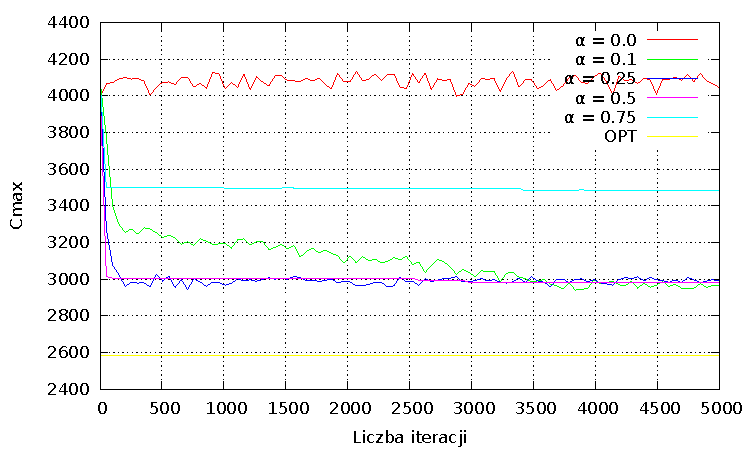
\includegraphics{./figures/inst01_rnd_alpha_smooth.pdf}
    \caption{$ \alpha = \{ 0.0, 0.1, 0.25, 0.5, 0.75 \} $}
\end{figure}

\newpage
\subsubsection{Grupa instancji 4}
Różne wartości parametru $q_0$.

\begin{center}
\begin{tabular}{|r|l|}
  \hline
  klasa instancji & losowa \\
  liczba zadań & 50 \\
  czasy operacji & $ \langle 5;100 \rangle $  \\
  liczba mrówek & 10 \\
  liczba pokoleń & 5000 \\
  $ \rho $ & 0.01 \\
  $ \beta $ & 2 \\
  $ \alpha $ & 0.1 \\
  $ \tau_0 $ & 0.001 \\
  \hline
\end{tabular}
\end{center}

\begin{figure}[h]
    \centering
    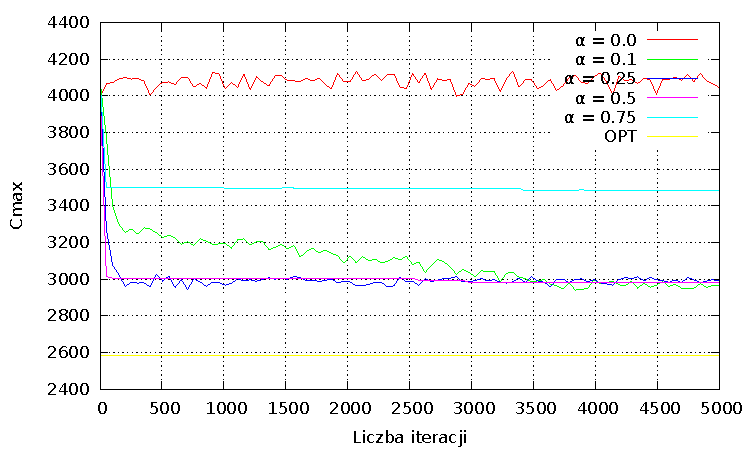
\includegraphics{./figures/inst01_rnd_alpha_smooth.pdf}
    \caption{$ q_0 = \{ 0.0, 0.25, 0.5, 0.75 \} $}
\end{figure}


\end{document}
